\documentclass[12pt]{article}

\usepackage[T1]{fontenc} \usepackage[icelandic]{babel}
\usepackage{latexsym,amssymb,amsmath}
\usepackage{pgfplots}
\usepackage{float}
\usepackage[absolute,overlay]{textpos}
\newcounter{marknumber}
\pgfplotsset{
    error bars/every nth mark/.style={
        /pgfplots/error bars/draw error bar/.prefix code={
            \pgfmathtruncatemacro\marknumbercheck{mod(floor(\themarknumber/2),#1)}
            \ifnum\marknumbercheck=0
            \else
                \begin{scope}[opacity=0]
            \fi
        },
        /pgfplots/error bars/draw error bar/.append code={
            \ifnum\marknumbercheck=0
            \else
                \end{scope}
            \fi
            \stepcounter{marknumber}    
        }
    }
}
\usepackage{graphicx}
\graphicspath{ {./html/} }
\usepackage{hyperref, color}
\hypersetup{
    colorlinks=true,
    linktoc=all,
    linkcolor=blue,
}

\begin{document}


\centerline{\bf \Huge EÐL207G Verkefni 4 RCL}
\centerline{\bf Mikael Sævar Scheving Eggertsson, Torfi Þorgrímsson}

\centerline{\bf \large }

\tableofcontents
\newpage
\section{}
\subsection{}
%3.1

$R_{innra}$ = 53ohm

\subsection{}
% 3.2 
\begin{table}[H]
    \begin{tabular}{|c|c|c|c|c|c|c|c|c|}
    \hline
    $V_R(t) [V]$  & 2.88 & 2.40 & 1.60 & 1.08 & 0.72 & 0.48 & 0.36 & 0.24  \\
    \hline
    t[$\mu s$] & 0 & 10 & 30 & 50 & 70 & 90 & 110 & 130  \\
    \hline
    \end{tabular}
\end{table}
 
%insert graf Vr af t
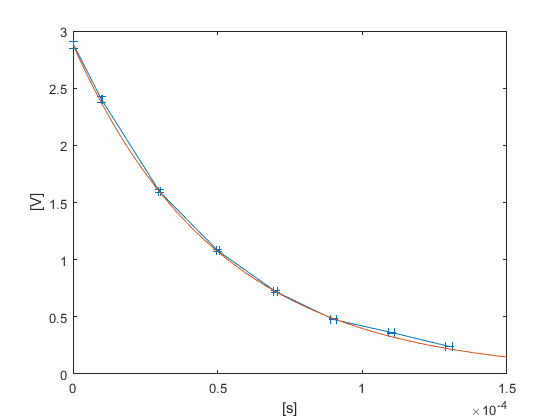
\includegraphics[scale=0.7]{data_01}

\subsection{}
% 3.3
\begin{table}[H]
    \begin{tabular}{|c|c|c|c|c|c|c|c|c|}
    \hline
    $V_R(t) [V]$  & 0.576 & -0.432 & 0.328 & -2.40 & 0.176 & -0.128 & 0.096 & -0.072 \\
    \hline
    t[$\mu s$]    & 16.0 & 48.0 & 79.5 & 112.0 & 142.0 & 173.5 & 204.5 & 236.5 \\
    \hline
    \end{tabular}
\end{table}


%insert graf n af t
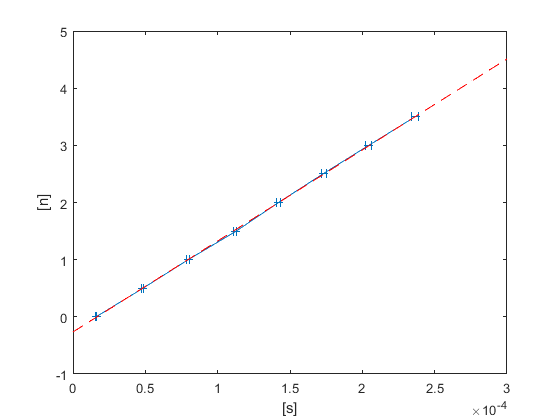
\includegraphics[scale=0.7]{data_03.png}

\end{document}